\section{Data Warehouse Modeling: Data Cube and OLAP}

% TODO: Example ERM for sales

\begin{frame}{From Tables and Spreadsheets to Data Cubes}
	\begin{itemize}
		\item Data warehouse is based on a \textbf{\color{airforceblue}multidimensional data model} which views data in the form of a \textbf{data cube}.
		\item A {\color{faugray}\textbf{data cube}} allows data (example: sales) to be modeled and viewed in multiple dimensions.
		      \begin{itemize}
			      \item Defined by dimension and facts.
			      \item \textbf{Dimension tables:} such as: \texttt{item (item\_name, brand, type)},\\
			            or: \texttt{time (day, week, month, quarter, year)}.
			      \item \textbf{Fact table:} Contains \textbf{measures} (such as \texttt{dollars\_sold}) and references (\texttt{foreign keys}) to each of the related dimension tables.
		      \end{itemize}
		\item \textbf{$n$-dimensional base cube.}
		      \begin{itemize}
			      \item Called a base cuboid in data warehousing literature.
		      \end{itemize}
		\item \textbf{Top most $0$-dimensional cuboid.}
		      \begin{itemize}
			      \item Holds the highest-level of summarization.
			      \item Called the apex cuboid.
		      \end{itemize}
		\item \textbf{Lattice of cuboids.} (Forms a data cube)
	\end{itemize}
\end{frame}

\begin{frame}{3-D Data Cube - Example}
	\begin{center}
		\scalebox{0.875}{
			\begin{tikzpicture}[scale=1]
				% Important: 
				% If the coordinates are x, y, z then:
				% x = 0 is the left side, x = 4 is the right side
				% y = 0 is the bottom side, y = 4 is the top side
				% z = 0 is the back side, z = 4 is the front side
				% 
				% To get the left bottom corner of the cube, use (0,0,4):
				% \fill[black] (0,0,4) circle (1.5pt);
				\useasboundingbox (-2.5,-1.8,4) rectangle (8,4,-1);

				% 1. STEP - Talking points:
				% - Imagine a three-dimensional coordinate system

				% Only axis
				\only<1-3>{
					\draw[->] (0,0,4) -- (0,5,4);
					\draw[->] (0,0,4) -- (5,0,4);
					\draw[->] (0,0,4) -- (0,0,-1);
				}

				% Axis labels
				\only<1-4>{
					\node[anchor=south,rotate=90] at (-0.25,2.5,4) {\texttt{Time}};
					\node[anchor=north] at (2.5,-0.25,4) {\texttt{Region}};
					\node[anchor=south,rotate=45] at (-0.125,0.125,1.5) {\texttt{Product}};
				}

				% 2. STEP - Talking points:
				% - Individual data points can be located anywhere in this coordinate system

				% Add data points with labels 
				\only<2-3>{
					\fill[black] (1.3,0.3,3.9) circle (1.5pt) node[above right] {\tiny{(Erlangen/Bavaria/Germany, 01/05/2023, Series 8/Washer) - (430€)}};
					\fill[black] (2.9,1.4,0.3) circle (1.5pt) node[above right] {\tiny{(Rome/Lazio/Italy, 23/06/2024, ePhone 16 Pro/Phone) - (1250€)}};
				}

				% Also add a lot more without labels 
				\only<3-6>{
					\fill[gray] (0.4,0.3,1.3) circle (1.5pt);
					\fill[gray] (0.5,1.9,1.8) circle (1.5pt);
					\fill[gray] (1.2,0.5,2.1) circle (1.5pt);
					\fill[gray] (1.5,0.8,2.4) circle (1.5pt);
					\fill[gray] (1.8,0.2,2.7) circle (1.5pt);
					\fill[gray] (2.1,1.6,1.0) circle (1.5pt);
					\fill[gray] (2.4,0.9,3.3) circle (1.5pt);
					\fill[gray] (2.7,3.2,3.6) circle (1.5pt);
					%\fill[gray] (1.0,1.5,3.9) circle (1.5pt);
					\fill[gray] (3.3,2.8,3.2) circle (1.5pt);
					\fill[gray] (3.6,2.1,3.5) circle (1.5pt);
					\fill[gray] (3.6,2.1,3.5) circle (1.5pt);
					\fill[gray] (3.9,1.4,4) circle (1.5pt);
					% ...
				}

				% 3. STEP - Talking points:
				% - All these data points can be grouped into a cube
				% - The facts (e.g. prices) of all the data points in the cube can be aggregated

				% Repetition of the axis (taking the cube into account)
				\only<4>{
					\draw[->] (0,0,4) -- (0,5,4);
					\draw[->] (0,0,4) -- (5,0,4);
					\draw[->, dashed] (0,0,4) -- (0,0,-1);
				}

				% Repetition of the previously labeled data points (now without labels)
				\only<4-6>{
					\fill[black] (1.3,0.3,3.9) circle (1.5pt);
					\fill[black] (2.9,1.4,0.3) circle (1.5pt);
				}

				% Cube
				\only<4>{
					\foreach \x in{0,4,...,4}
						{   \draw (0,\x ,4) -- (4,\x ,4);
							\draw (\x ,0,4) -- (\x ,4,4);
							\draw (4,\x ,4) -- (4,\x ,0);
							\draw (\x ,4,4) -- (\x ,4,0);
							\draw (4,0,\x ) -- (4,4,\x );
							\draw (0,4,\x ) -- (4,4,\x );
						}
				}

				% 4. STEP - Talking points:
				% - The cube can be sliced into smaller cubes for more detailed analysis
				% - There aggregation on the facts of a smaller cube can be performed

				% Highest granularity cube
				\only<5>{
					\foreach \x in{0,...,4}
						{   \draw (0,\x ,4) -- (4,\x ,4);
							\draw (\x ,0,4) -- (\x ,4,4);
							\draw (4,\x ,4) -- (4,\x ,0);
							\draw (\x ,4,4) -- (\x ,4,0);
							\draw (4,0,\x ) -- (4,4,\x );
							\draw (0,4,\x ) -- (4,4,\x );
						}
				}

				% Axis categories (highest granularity)
				\only<5>{
					% Time axis
					\node[anchor=east] at (-0.25,0.5,4) {\texttt{2023}};
					\node[anchor=east] at (-0.25,1.5,4) {\texttt{2024}};
					\node[anchor=east] at (-0.25,2.5,4) {\texttt{2025}};
					\node[anchor=east] at (-0.25,3.5,4) {\texttt{2026}};

					% Region axis 
					\node[anchor=east,rotate=90] at (0.5, -0.25, 4) {\texttt{France}};
					\node[anchor=east,rotate=90] at (1.5, -0.25, 4) {\texttt{Germany}};
					\node[anchor=east,rotate=90] at (2.5, -0.25, 4) {\texttt{Italy}};
					\node[anchor=east,rotate=90] at (3.5, -0.25, 4) {\texttt{Spain}};

					% Product axis
					\node[anchor=west,rotate=315] at (4.125, -0.125, 3.5) {\texttt{Washer}};
					\node[anchor=west,rotate=315] at (4.125, -0.125, 2.5) {\texttt{Fridge}};
					\node[anchor=west,rotate=315] at (4.125, -0.125, 1.5) {\texttt{TV}};
					\node[anchor=west,rotate=315] at (4.125, -0.125, 0.5) {\texttt{Phone}};
				}

				% 5. STEP - Talking points:
				% - The cube can be even be sliced into smaller cubes for more detailed analysis
				% - In this example we only go to the next granularity level in the time dimension
				% - The other dimensions also have finer granularity levels
				% - More on this on a later slide

				% Next granularity cube
				\only<6>{
					\foreach \y in{0,0.25,...,4}
						{
							\foreach \xz in{0,1,...,4}
								{   \draw (0,\y ,4) -- (4,\y ,4);
									\draw (\xz ,0,4) -- (\xz ,4,4);
									\draw (4,\y ,4) -- (4,\y ,0);
									\draw (\xz ,4,4) -- (\xz ,4,0);
									\draw (4,0,\xz ) -- (4,4,\xz );
									\draw (0,4,\xz ) -- (4,4,\xz );
								}
						}
				}

				% Axis categories (highest granularity)
				\only<6>{
					% Time axis
					\node[anchor=east] at (-1.25,0.5,4) {\texttt{2023}};
					\node[anchor=east] at (-0.25,0.125,4) {\small{\texttt{Q1}}};
					\node[anchor=east] at (-0.25,0.375,4) {\small{\texttt{Q2}}};
					\node[anchor=east] at (-0.25,0.625,4) {\small{\texttt{Q3}}};
					\node[anchor=east] at (-0.25,0.875,4) {\small{\texttt{Q4}}};
					\node[anchor=east] at (-1.25,1.5,4) {\texttt{2024}};
					\node[anchor=east] at (-0.25,1.125,4) {\small{\texttt{Q1}}};
					\node[anchor=east] at (-0.25,1.375,4) {\small{\texttt{Q2}}};
					\node[anchor=east] at (-0.25,1.625,4) {\small{\texttt{Q3}}};
					\node[anchor=east] at (-0.25,1.875,4) {\small{\texttt{Q4}}};
					\node[anchor=east] at (-1.25,2.5,4) {\texttt{2025}};
					\node[anchor=east] at (-0.25,2.125,4) {\small{\texttt{Q1}}};
					\node[anchor=east] at (-0.25,2.375,4) {\small{\texttt{Q2}}};
					\node[anchor=east] at (-0.25,2.625,4) {\small{\texttt{Q3}}};
					\node[anchor=east] at (-0.25,2.875,4) {\small{\texttt{Q4}}};
					\node[anchor=east] at (-1.25,3.5,4) {\texttt{2026}};
					\node[anchor=east] at (-0.25,3.125,4) {\small{\texttt{Q1}}};
					\node[anchor=east] at (-0.25,3.375,4) {\small{\texttt{Q2}}};
					\node[anchor=east] at (-0.25,3.625,4) {\small{\texttt{Q3}}};
					\node[anchor=east] at (-0.25,3.875,4) {\small{\texttt{Q4}}};

					% Region axis 
					\node[anchor=east,rotate=90] at (0.5, -0.25, 4) {\texttt{France}};
					\node[anchor=east,rotate=90] at (1.5, -0.25, 4) {\texttt{Germany}};
					\node[anchor=east,rotate=90] at (2.5, -0.25, 4) {\texttt{Italy}};
					\node[anchor=east,rotate=90] at (3.5, -0.25, 4) {\texttt{Spain}};

					% Product axis
					\node[anchor=west,rotate=315] at (4.125, -0.125, 3.5) {\texttt{Washer}};
					\node[anchor=west,rotate=315] at (4.125, -0.125, 2.5) {\texttt{Fridge}};
					\node[anchor=west,rotate=315] at (4.125, -0.125, 1.5) {\texttt{TV}};
					\node[anchor=west,rotate=315] at (4.125, -0.125, 0.5) {\texttt{Phone}};
				}


			\end{tikzpicture}
		}
	\end{center}
\end{frame}

\begin{frame}{From Tables and Spreadsheets to Data Cubes}
	\begin{itemize}
		\item Data warehouse is based on a \textbf{\color{airforceblue}multidimensional data model} which views data in the form of a \textbf{data cube}.
		\item A {\color{faugray}\textbf{data cube}} allows data (example: sales) to be modeled and viewed in multiple dimensions.
		      \begin{itemize}
			      \item Defined by dimension and facts.
			      \item \textbf{Dimension tables:} such as: \texttt{item (item\_name, brand, type)},\\
			            or: \texttt{time (day, week, month, quarter, year)}.
			      \item \textbf{Fact table:} Contains \textbf{measures} (such as \texttt{dollars\_sold}) and references (\texttt{foreign keys}) to each of the related dimension tables.
		      \end{itemize}
		\item \textbf{$n$-dimensional base cube.}
		      \begin{itemize}
			      \item Called a base cuboid in data warehousing literature.
		      \end{itemize}
		\item \textbf{Top most $0$-dimensional cuboid.}
		      \begin{itemize}
			      \item Holds the highest-level of summarization.
			      \item Called the apex cuboid.
		      \end{itemize}
		\item \textbf{Lattice of cuboids.} (Forms a data cube)
	\end{itemize}
\end{frame}

\begin{frame}{Cube: A Lattice of Cuboids}
	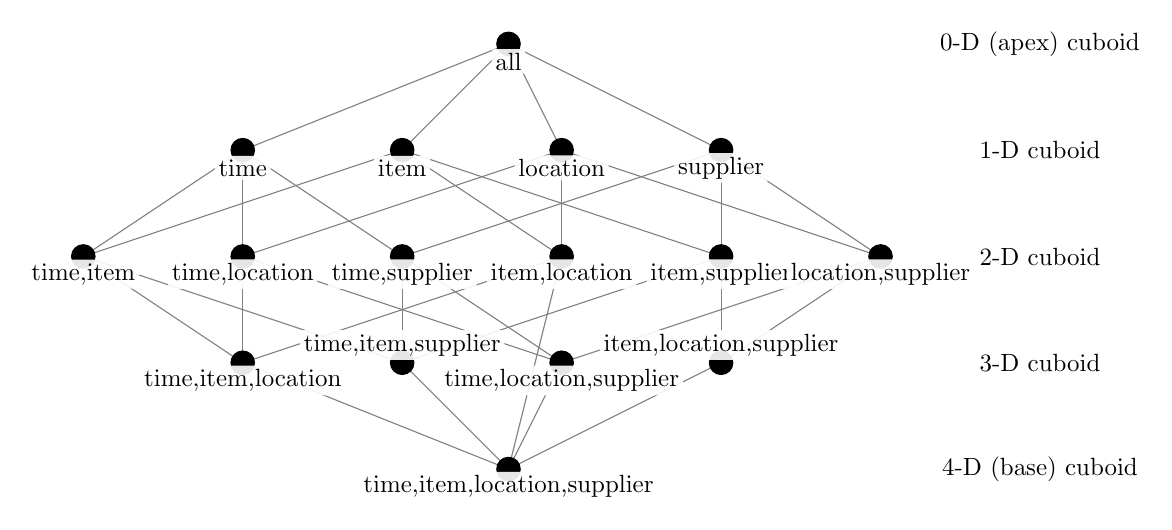
\begin{tikzpicture}[
			scale=0.9,
			every node/.style={transform shape}
		]
		% Connections
		\draw[gray] (3,6) -- (-0.75,4.5);
		\draw[gray] (3,6) -- (1.5,4.5);
		\draw[gray] (3,6) -- (3.75,4.5);
		\draw[gray] (3,6) -- (6,4.5);

		\draw[gray] (-0.75,4.5) -- (-3,3);
		\draw[gray] (-0.75,4.5) -- (-0.75,3);
		\draw[gray] (-0.75,4.5) -- (1.5,3);
		\draw[gray] (1.5,4.5) -- (-3,3);
		\draw[gray] (1.5,4.5) -- (3.75,3);
		\draw[gray] (1.5,4.5) -- (6,3);
		\draw[gray] (3.75,4.5) -- (-0.75,3);
		\draw[gray] (3.75,4.5) -- (3.75,3);
		\draw[gray] (3.75,4.5) -- (8.25,3);
		\draw[gray] (6,4.5) -- (1.5,3);
		\draw[gray] (6,4.5) -- (6,3);
		\draw[gray] (6,4.5) -- (8.25,3);

		\draw[gray] (-3,3) -- (-0.75,1.5);
		\draw[gray] (-3,3) -- (1.5,1.5);
		\draw[gray] (-0.75,3) -- (-0.75,1.5);
		\draw[gray] (-0.75,3) -- (3.75,1.5);
		\draw[gray] (1.5,3) -- (1.5,1.5);
		\draw[gray] (1.5,3) -- (3.75,1.5);
		\draw[gray] (3.75,3) -- (-0.75,1.5);
		\draw[gray] (3.75,3) -- (3,0);
		\draw[gray] (6,3) -- (1.5,1.5);
		\draw[gray] (6,3) -- (6,1.5);
		\draw[gray] (8.25,3) -- (3.75,1.5);
		\draw[gray] (8.25,3) -- (6,1.5);

		\draw[gray] (-0.75,1.5) -- (3,0);
		\draw[gray] (1.5,1.5) -- (3,0);
		\draw[gray] (3.75,1.5) -- (3,0);
		\draw[gray] (6,1.5) -- (3,0);

		% Nodes
		\node[draw, circle, fill=black] at (3,6) {};
		\node[draw, circle, fill=black] at (-0.75,4.5) {};
		\node[draw, circle, fill=black] at (1.5,4.5) {};
		\node[draw, circle, fill=black] at (3.75,4.5) {};
		\node[draw, circle, fill=black] at (6,4.5) {};

		\node[draw, circle, fill=black] at (-3,3) {};
		\node[draw, circle, fill=black] at (-0.75,3) {};
		\node[draw, circle, fill=black] at (1.5,3) {};
		\node[draw, circle, fill=black] at (3.75,3) {};
		\node[draw, circle, fill=black] at (6,3) {};
		\node[draw, circle, fill=black] at (8.25,3) {};

		\node[draw, circle, fill=black] at (-0.75,1.5) {};
		\node[draw, circle, fill=black] at (1.5,1.5) {};
		\node[draw, circle, fill=black] at (3.75,1.5) {};
		\node[draw, circle, fill=black] at (6,1.5) {};

		\node[draw, circle, fill=black] at (3,0) {};

		% Labels
		\node[fill=white, text opacity=1, fill opacity=0.9, inner sep=1.5pt, rounded corners=1pt] at (3,5.75) {all};

		\node[fill=white, text opacity=1, fill opacity=0.9, inner sep=1.5pt, rounded corners=1pt] at (-0.75,4.25) {time};
		\node[fill=white, text opacity=1, fill opacity=0.9, inner sep=1.5pt, rounded corners=1pt] at (1.5,4.25) {item};
		\node[fill=white, text opacity=1, fill opacity=0.9, inner sep=1.5pt, rounded corners=1pt] at (3.75,4.25) {location};
		\node[fill=white, text opacity=1, fill opacity=0.9, inner sep=1.5pt, rounded corners=1pt] at (6,4.25) {supplier};

		\node[fill=white, text opacity=1, fill opacity=0.9, inner sep=1.5pt, rounded corners=1pt] at (-3,2.75) {time,item};
		\node[fill=white, text opacity=1, fill opacity=0.9, inner sep=1.5pt, rounded corners=1pt] at (-0.75,2.75) {time,location};
		\node[fill=white, text opacity=1, fill opacity=0.9, inner sep=1.5pt, rounded corners=1pt] at (1.5,2.75) {time,supplier};
		\node[fill=white, text opacity=1, fill opacity=0.9, inner sep=1.5pt, rounded corners=1pt] at (3.75,2.75) {item,location};
		\node[fill=white, text opacity=1, fill opacity=0.9, inner sep=1.5pt, rounded corners=1pt] at (6,2.75) {item,supplier};
		\node[fill=white, text opacity=1, fill opacity=0.9, inner sep=1.5pt, rounded corners=1pt] at (8.25,2.75) {location,supplier};

		\node[fill=white, text opacity=1, fill opacity=0.9, inner sep=1.5pt, rounded corners=1pt] at (-0.75,1.25) {time,item,location};
		\node[fill=white, text opacity=1, fill opacity=0.9, inner sep=1.5pt, rounded corners=1pt] at (1.5,1.75) {time,item,supplier};
		\node[fill=white, text opacity=1, fill opacity=0.9, inner sep=1.5pt, rounded corners=1pt] at (3.75,1.25) {time,location,supplier};
		\node[fill=white, text opacity=1, fill opacity=0.9, inner sep=1.5pt, rounded corners=1pt] at (6,1.75) {item,location,supplier};

		\node[fill=white, text opacity=1, fill opacity=0.9, inner sep=1.5pt, rounded corners=1pt] at (3,-0.25) {time,item,location,supplier};

		% Cuboid labels
		\node[fill=white, text opacity=1, fill opacity=0.9, inner sep=1.5pt, rounded corners=1pt] at (10.5,6) {$0$-D (apex) cuboid};
		\node[fill=white, text opacity=1, fill opacity=0.9, inner sep=1.5pt, rounded corners=1pt] at (10.5,4.5) {$1$-D cuboid};
		\node[fill=white, text opacity=1, fill opacity=0.9, inner sep=1.5pt, rounded corners=1pt] at (10.5,3) {$2$-D cuboid};
		\node[fill=white, text opacity=1, fill opacity=0.9, inner sep=1.5pt, rounded corners=1pt] at (10.5,1.5) {$3$-D cuboid};
		\node[fill=white, text opacity=1, fill opacity=0.9, inner sep=1.5pt, rounded corners=1pt] at (10.5,0) {$4$-D (base) cuboid};
	\end{tikzpicture}
\end{frame}

\begin{frame}{Conceptual Modeling of Data Warehouses}
	\begin{enumerate}
		\item \textbf{Star schema:}.
		      \begin{itemize}
			      \item A fact table in the middle connected to a set of dimension tables.
		      \end{itemize}
		\item \textbf{Snowflake schema:}.
		      \begin{itemize}
			      \item A refinement of the star schema where some dimensional hierarchies \\
			            are \textbf{normalized} into a set of smaller dimension tables,\\
			            forming a shape similar to a snowflake.
			      \item I. e. dimension tables of a star schema are split into multiple (dimension) tables\\ along their respective granularity level, but not split/normalized for every granularity.
		      \end{itemize}
		\item \textbf{Fact constellations:}.
		      \begin{itemize}
			      \item Multiple fact tables sharing dimension tables, \\
			            viewed as a collection of stars, therefore called \\
			            \textbf{galaxy schema} or fact constellation.
		      \end{itemize}
	\end{enumerate}
\end{frame}

\begin{frame}{Example of a Star Schema}
	\begin{center}
		\begin{tikzpicture}
			\node[basic, rectangle split part fill={green!20,white}] at (2,2) (time) {time
				\nodepart{second}
				\underline{time\_key}\\
				day\\
				day\_of\_week\\
				month\\
				quarter\\
				year};

			\node[basic] at (2,-1.5) (branch) {branch
				\nodepart{second}
				\underline{branch\_key}\\
				branch\_name\\
				branch\_type};

			\node[basic, rectangle split part fill={orange!20,white}] at (12,2) (item) {item
				\nodepart{second}
				\underline{item\_key}\\
				item\_name\\
				brand\\
				type\\
				supplier\_type};

			\node[basic, rectangle split part fill={yellow!20,white}] at (12,-1.25) (location) {location
				\nodepart{second}
				\underline{location\_key}\\
				street\\
				city\\
				province\\
				country};

			\node[] at (7,3) {Sales fact table:};
			\node[fill=green!20, minimum width = 3cm, minimum height=0.5cm, align=right] at (7,2.5) (a) {time\_key};
			\node[fill=orange!20, minimum width = 3cm, minimum height=0.5cm, align=right] at (7,2) (b) {item\_key};
			\node[fill=blue!20, minimum width = 3cm, minimum height=0.5cm, align=right] at (7,1.5) (c) {branch\_key};
			\node[fill=yellow!20, minimum width = 3cm, minimum height=0.5cm, align=right] at (7,1) (d) {location\_key};
			\node[fill=red!20, minimum width = 3cm, minimum height=0.5cm, align=right] at (7,0.5) (units) {units\_sold};
			\node[fill=red!20, minimum width = 3cm, minimum height=0.5cm, align=right] at (7,0) (dollars) {dollars\_sold};
			\node[fill=red!20, minimum width = 3cm, minimum height=0.5cm, align=right] at (7,-0.5) (sales) {avg\_sales};
			\draw[->, dashed] (a.west) -- (time);
			\draw[->, dashed] (b) -- (item);
			\draw[->, dashed] (c.west) -- (branch);
			\draw[->, dashed] (d.east) -- (location);

			\node[fill=red!20, minimum width = 3cm, minimum height=0.5cm, align=right] at (5,-1.5) (e) {Measures};
			\draw[-] (e) -- (units.west);
			\draw[-] (e) -- (dollars.west);
			\draw[-] (e) -- (sales.west);
		\end{tikzpicture}
	\end{center}
\end{frame}

\begin{frame}{Example of Snowflake Schema}
	\begin{center}
		\begin{tikzpicture}
			\node[basic, rectangle split part fill={green!20,white}] at (2,2) (time) {time
				\nodepart{second}
				\underline{time\_key}\\
				day\\
				day\_of\_week\\
				month\\
				quarter\\
				year};

			\node[basic] at (2,-1.5) (branch) {branch
				\nodepart{second}
				\underline{branch\_key}\\
				branch\_name\\
				branch\_type};

			\node[basic, rectangle split part fill={orange!20,white}] at (10,2) (item) {item
				\nodepart{second}
				\underline{item\_key}\\
				item\_name\\
				brand\\
				type\\
				supplier\_key};

			\node[basic, rectangle split part fill={orange!20,white}] at (13,2) (supplier) {supplier
				\nodepart{second}
				\underline{supplier\_key}\\
				supplier\_type};

			\node[basic, rectangle split part fill={yellow!20,white}] at (10,-1.25) (location) {location
				\nodepart{second}
				\underline{location\_key}\\
				street\\
				city\_key};

			\node[basic, rectangle split part fill={yellow!20,white}] at (13,-1.5) (city) {city
				\nodepart{second}
				\underline{city\_key}\\
				city\\
				province\\
				country};

			\node[] at (6,3) {Sales fact table:};
			\node[fill=green!20, minimum width = 3cm, minimum height=0.5cm, align=right] at (6,2.5) (a) {time\_key};
			\node[fill=orange!20, minimum width = 3cm, minimum height=0.5cm, align=right] at (6,2) (b) {item\_key};
			\node[fill=blue!20, minimum width = 3cm, minimum height=0.5cm, align=right] at (6,1.5) (c) {branch\_key};
			\node[fill=yellow!20, minimum width = 3cm, minimum height=0.5cm, align=right] at (6,1) (d) {location\_key};
			\node[fill=red!20, minimum width = 3cm, minimum height=0.5cm, align=right] at (6,0.5) (units) {units\_sold};
			\node[fill=red!20, minimum width = 3cm, minimum height=0.5cm, align=right] at (6,0) (dollars) {dollars\_sold};
			\node[fill=red!20, minimum width = 3cm, minimum height=0.5cm, align=right] at (6,-0.5) (sales) {avg\_sales};
			\draw[->, dashed] (a.west) -- (time) ;
			\draw[->, dashed] (b) -- (item) ;
			\draw[->, dashed] (c.west) -- (branch) ;
			\draw[->, dashed] (d.east) -- (location) ;
			\draw[->, dashed] (10,-2) -- (city) ;
			\draw[->, dashed] (11,1) -- (supplier) ;

			\node[fill=red!20, minimum width = 3cm, minimum height=0.5cm, align=right] at (5,-1.5) (e) {Measures};
			\draw[-] (e.north west) -- (units.west);
			\draw[-] (e.north west) -- (dollars.west);
			\draw[-] (e.north west) -- (sales.west);
		\end{tikzpicture}
	\end{center}
\end{frame}

\begin{frame}{Example of Fact Constellation}
	\vspace{-2.4em}
	\tikzset{basic/.style={
				draw,
				rectangle split,
				rectangle split parts=2,
				rectangle split part fill={blue!20,white},
				minimum width=2.5cm,
				text width=2cm,
				align=left,
				font=\itshape
			},
		Diamond/.style={ diamond,
				draw,
				shape aspect=2,
				inner sep = 2pt,
				text centered,
				fill=blue!10!white,
				font=\itshape
			}}
	\begin{center}
		\begin{tikzpicture}[scale=0.9,every node/.style={transform shape}]
			\node[basic, rectangle split part fill={green!20,white}] at (2,2) (time) {time
				\nodepart{second}
				\underline{time\_key}\\
				day\\
				day\_of\_week\\
				month\\
				quarter\\
				year};

			\node[basic] at (2,-1.5) (branch) {branch
				\nodepart{second}
				\underline{branch\_key}\\
				branch\_name\\
				branch\_type};

			\node[basic, rectangle split part fill={orange!20,white}] at (10,2) (item) {item
				\nodepart{second}
				\underline{item\_key}\\
				item\_name\\
				brand\\
				type\\
				supplier\_type};

			\node[basic, rectangle split part fill={yellow!20,white}] at (10,-1.25) (location) {location
				\nodepart{second}
				\underline{location\_key}\\
				street\\
				city\\
				province\\
				country};

			\node[basic, rectangle split part fill={blue!20,white}] at (13.5,-2) (shipper) {shipper
				\nodepart{second}
				\underline{shipper\_key}\\
				shipper\_name\\
				location\_key\\
				shipper\_type};

			\node[] at (6,3) {Sales fact table:};
			\node[fill=green!20, minimum width = 3cm, minimum height=0.5cm, align=right] at (6,2.5) (a) {time\_key};
			\node[fill=orange!20, minimum width = 3cm, minimum height=0.5cm, align=right] at (6,2) (b) {item\_key};
			\node[fill=blue!20, minimum width = 3cm, minimum height=0.5cm, align=right] at (6,1.5) (c) {branch\_key};
			\node[fill=yellow!20, minimum width = 3cm, minimum height=0.5cm, align=right] at (6,1) (d) {location\_key};
			\node[fill=red!20, minimum width = 3cm, minimum height=0.5cm, align=right] at (6,0.5) (units) {units\_sold};
			\node[fill=red!20, minimum width = 3cm, minimum height=0.5cm, align=right] at (6,0) (dollars) {dollars\_sold};
			\node[fill=red!20, minimum width = 3cm, minimum height=0.5cm, align=right] at (6,-0.5) (sales) {avg\_sales};
			\draw[->, dashed] (a.west) -- (time) ;
			\draw[->, dashed] (b) -- (item) ;
			\draw[->, dashed] (c.west) -- (branch) ;
			\draw[->, dashed] (d.east) -- (location) ;


			\node[] at (13.5,3) {Shipping fact table:};
			\node[fill=green!20, minimum width = 3cm, minimum height=0.5cm, align=right] at (13.5,2.5) (q) {time\_key};
			\node[fill=orange!20, minimum width = 3cm, minimum height=0.5cm, align=right] at (13.5,2) (w) {item\_key};
			\node[fill=blue!20, minimum width = 3cm, minimum height=0.5cm, align=right] at (13.5,1.5) (e) {shipper\_key};
			\node[fill=yellow!20, minimum width = 3cm, minimum height=0.5cm, align=right] at (13.5,1) (r) {from\_location};
			\node[fill=yellow!20, minimum width = 3cm, minimum height=0.5cm, align=right] at (13.5,0.5) (t) {to\_location};
			\node[fill=red!20, minimum width = 3cm, minimum height=0.5cm, align=right] at (13.5,0) (z) {dollars\_cost};
			\node[fill=red!20, minimum width = 3cm, minimum height=0.5cm, align=right] at (13.5,-0.5) (u) {units\_shipped};
			\draw[->, dashed] (q) to [out=160,in=30] (time) ;
			\draw[->, dashed] (w) -- (item) ;
			\draw[->, dashed] (e.east) to [out=0,in=30] (shipper) ;
			\draw[->, dashed] (r.west) -- (location);
			\draw[->, dashed] (t.west) -- (location);
			\draw[->, dashed] (shipper) -- (location);

			\node[fill=red!20, minimum width = 3cm, minimum height=0.5cm, align=right] at (5,-1.5) (e) {Measures};
			\draw[-] (e.north west) -- (units.west);
			\draw[-] (e.north west) -- (dollars.west);
			\draw[-] (e.north west) -- (sales.west);
		\end{tikzpicture}
	\end{center}
\end{frame}

\begin{frame}{A Concept Hierarchy: Dimension (Location)}
	\begin{center}
		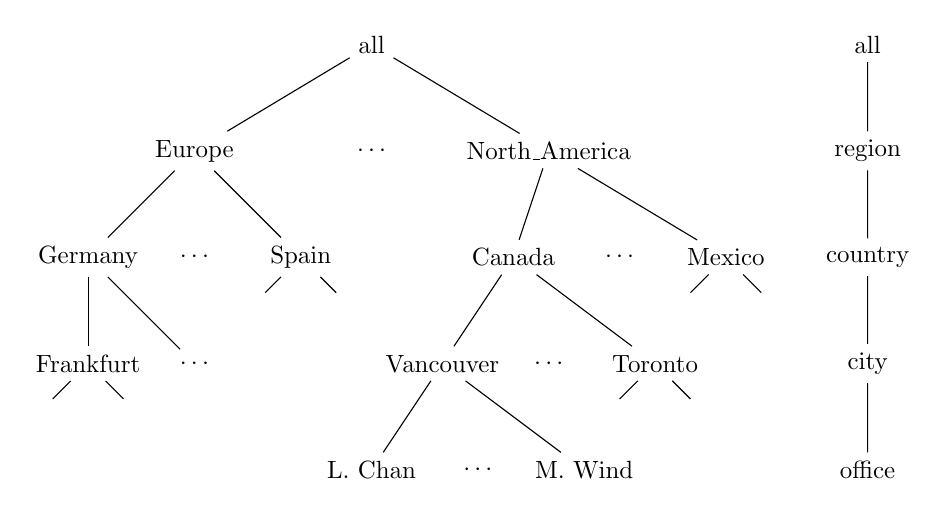
\begin{tikzpicture}[scale=0.9,every node/.style={transform shape}]
			\node at (2,6) (all) {all};

			\node at (-0.5,4.5) (europe) {Europe};
			\node at (2,4.5) (dot1) {$\cdots$};
			\node at (4.5,4.5) (america) {North\_America};

			\node at (-2,3) (germany) {Germany};
			\node at (-0.5,3) (dots2) {$\cdots$};
			\node at (1,3) (spain) {Spain};
			\node at (4,3) (canada) {Canada};
			\node at (5.5,3) (dots3) {$\cdots$};
			\node at (7,3) (mexico) {Mexico};

			\node at (-2,1.5) (frankfurt) {Frankfurt};
			\node at (-0.5,1.5) (dots4) {$\cdots$};
			\node at (3,1.5) (vancouver) {Vancouver};
			\node at (4.5,1.5) (dots5) {$\cdots$};
			\node at (6,1.5) (toronto) {Toronto};
			\node at (2,0) (lchan) {L. Chan};
			\node at (3.5,0) (dots6) {$\cdots$};
			\node at (5,0) (mwind) {M. Wind};

			\draw (all) -- (europe);
			\draw (all) -- (america);
			\draw (europe) -- (germany);
			\draw (europe) -- (spain);
			\draw (america) -- (canada);
			\draw (america) -- (mexico);
			\draw (germany) -- (frankfurt);
			\draw (germany) -- (dots4);
			\draw (spain) -- (0.5,2.5);
			\draw (spain) -- (1.5,2.5);
			\draw (mexico) -- (6.5,2.5);
			\draw (mexico) -- (7.5,2.5);
			\draw (frankfurt) -- (-2.5,1);
			\draw (frankfurt) -- (-1.5,1);
			\draw (toronto) -- (5.5,1);
			\draw (toronto) -- (6.5,1);
			\draw (canada) -- (vancouver);
			\draw (canada) -- (toronto);
			\draw (vancouver) -- (lchan);
			\draw (vancouver) -- (mwind);

			\node at (9,6) (all2) {all};
			\node at (9,4.5) (region2)  {region};
			\node at (9,3) (country2) {country};
			\node at (9,1.5) (city2) {city};
			\node at (9,0) (office2) {office};
			\draw (all2) -- (region2);
			\draw (region2) -- (country2);
			\draw (country2) -- (city2);
			\draw (city2) -- (office2);
		\end{tikzpicture}
	\end{center}
\end{frame}

\begin{frame}{Data-Cube Measures}
	\begin{block}{Data-Cube Measure}
		A \textit{data-cube measure}, also called a \textit{fact}, is a numeric
		function that can be evaluated at each point in the data cube space.
	\end{block}

	\textbf{Three Categories:}
	\begin{enumerate}
		\item {\color{faugray}\textbf{Distributive:}}
		      \begin{itemize}
			      \item If the result derived by applying the function to the $n$ aggregate values obtained for $n$ partitions of the dataset is the same as that derived by applying the function on all the data without partitioning.\\
			            E.g. \texttt{COUNT, SUM, MIN, MAX}.
		      \end{itemize}
		\item {\color{faugray}\textbf{Algebraic:}}
		      \begin{itemize}
			      \item If it can be computed by an algebraic function with $M$ arguments, each of which is obtained by applying a distributive aggregate function.\\
			            E.g. \texttt{AVG, MIN$_N$, STD}.
		      \end{itemize}
		\item {\color{faugray}\textbf{Holistic:}}
		      \begin{itemize}
			      \item If there is no constant bound on the storage size needed to describe a subaggregate.\\
			            E.g. \texttt{MEDIAN, MODE, RANK}.
		      \end{itemize}
	\end{enumerate}
\end{frame}

\begin{frame}{Aggregation Type}
	\begin{itemize}
		\item \textbf{Non-trivial property.}
		      \begin{itemize}
			      \item Next to name and value range.
		      \end{itemize}
		\item \textbf{Defines the set of aggregation operations that can be executed on a measure (a fact).}
		\item \textbf{\color{airforceblue}STOCK:} Measure at a specific point in time.
		      \begin{itemize}
			      \item Aggregated as desired.
			      \item E.g. sales turnover, quantity of an item ordered per day.
		      \end{itemize}
		\item \textbf{\color{airforceblue}FLOW:} Measure over a period of time.
		      \begin{itemize}
			      \item Aggregated as desired, but temporal aggregation not permitted.
			      \item E.g. total stock and total inventory. Yet, summarization of article stock over multiple days makes no sense!
		      \end{itemize}
		\item \textbf{\color{airforceblue}VPU (Value per Unit):} Measures that cannot be summed.
		      \begin{itemize}
			      \item E.g. unit price, tax rates, exchange rates.
		      \end{itemize}
		\item \textbf{Always applicable: \texttt{MIN}, \texttt{MAX} and \texttt{AVG}.}
	\end{itemize}
\end{frame}

\begin{frame}{Aggregation Type}
	\textbf{Sales volume as a function of product, month, and region.}
	\begin{itemize}
		\item Dimensions: \texttt{Product, Location, Time.}
		\item Hierarchical summarization paths.
	\end{itemize}
	\vspace{0.5cm}
	\hspace{0.5cm}
	\begin{center}
		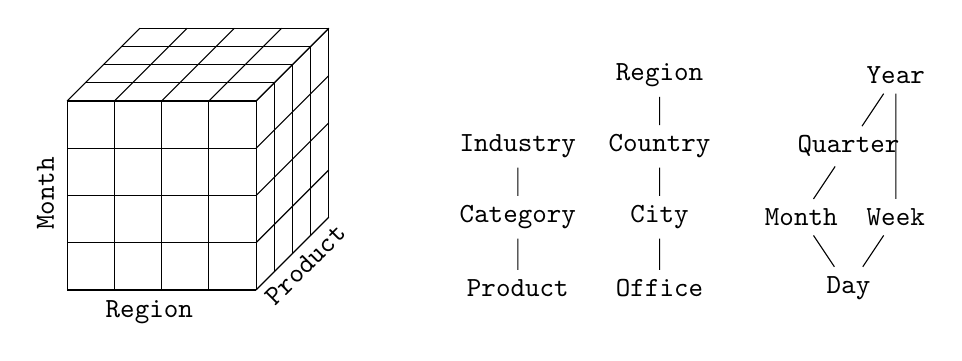
\begin{tikzpicture}[scale=0.6]
			\foreach \x in{0,...,4}
				{   \draw (0,\x ,4) -- (4,\x ,4);
					\draw (\x ,0,4) -- (\x ,4,4);
					\draw (4,\x ,4) -- (4,\x ,0);
					\draw (\x ,4,4) -- (\x ,4,0);
					\draw (4,0,\x ) -- (4,4,\x );
					\draw (0,4,\x ) -- (4,4,\x );
				}

			\node at (0.2,-2) {\texttt{Region}};
			\node[rotate=45] at (3.5,-1) {\texttt{Product}};
			\node[rotate=90] at (-2,0.5) {\texttt{Month}};

			\node at (8,1.5) (industry) {\texttt{Industry}};
			\node at (8,0) (category) {\texttt{Category}};
			\node at (8,-1.5) (product) {\texttt{Product}};
			\draw (industry) -- (category) -- (product);

			\node at (11,3) (region) {\texttt{Region}};
			\node at (11,1.5) (country) {\texttt{Country}};
			\node at (11,0) (city) {\texttt{City}};
			\node at (11,-1.5) (office) {\texttt{Office}};
			\draw (region) -- (country) -- (city) -- (office);

			\node at (16,3) (year) {\texttt{Year}};
			\node at (15,1.5) (quarter) {\texttt{Quarter}};
			\node at (14,0) (month) {\texttt{Month}};
			\node at (16,0) (week) {\texttt{Week}};
			\node at (15,-1.5) (day) {\texttt{Day}};
			\draw (year) -- (quarter) -- (month) -- (day) -- (week) -- (year);
		\end{tikzpicture}
	\end{center}
\end{frame}

\begin{frame}{Data Cube Sample}
	\centering
	\includegraphics[width=10cm,height=6cm]{img/datacube.pdf}
\end{frame}

\begin{frame}{Cuboids Corresponding to the Cube}
	\centering
	\vspace*{0.75cm}
	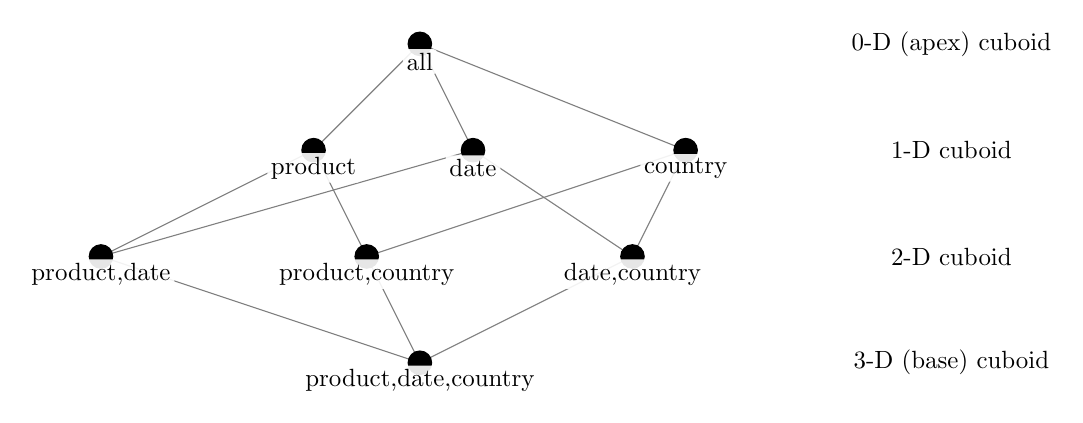
\begin{tikzpicture}[
			scale=0.9,
			every node/.style={transform shape}
		]
		% Connections
		\draw[gray] (3,6) -- (1.5,4.5);
		\draw[gray] (3,6) -- (3.75,4.5);
		\draw[gray] (3,6) -- (6.75,4.5);
		\draw[gray] (1.5,4.5) -- (-1.5,3);
		\draw[gray] (1.5,4.5) -- (2.25,3);
		\draw[gray] (3.75,4.5) -- (-1.5,3);
		\draw[gray] (3.75,4.5) -- (6,3);
		\draw[gray] (6.75,4.5) -- (2.25,3);
		\draw[gray] (6.75,4.5) -- (6,3);
		\draw[gray] (-1.5,3) -- (3,1.5);
		\draw[gray] (2.25,3) -- (3,1.5);
		\draw[gray] (6,3) -- (3,1.5);

		% Nodes
		\node[draw, circle, fill=black] at (3,6) {};
		\node[draw, circle, fill=black] at (1.5,4.5) {};
		\node[draw, circle, fill=black] at (3.75,4.5) {};
		\node[draw, circle, fill=black] at (6.75,4.5) {};
		\node[draw, circle, fill=black] at (-1.5,3) {};
		\node[draw, circle, fill=black] at (2.25,3) {};
		\node[draw, circle, fill=black] at (6,3) {};
		\node[draw, circle, fill=black] at (3,1.5) {};

		% Labels
		\node[fill=white, text opacity=1, fill opacity=0.9, inner sep=1.5pt, rounded corners=1pt] at (3,5.75) {all};

		\node[fill=white, text opacity=1, fill opacity=0.9, inner sep=1.5pt, rounded corners=1pt] at (1.5,4.25) {product};
		\node[fill=white, text opacity=1, fill opacity=0.9, inner sep=1.5pt, rounded corners=1pt] at (3.75,4.25) {date};
		\node[fill=white, text opacity=1, fill opacity=0.9, inner sep=1.5pt, rounded corners=1pt] at (6.75,4.25) {country};

		\node[fill=white, text opacity=1, fill opacity=0.9, inner sep=1.5pt, rounded corners=1pt] at (-1.5,2.75) {product,date};
		\node[fill=white, text opacity=1, fill opacity=0.9, inner sep=1.5pt, rounded corners=1pt] at (2.25,2.75) {product,country};
		\node[fill=white, text opacity=1, fill opacity=0.9, inner sep=1.5pt, rounded corners=1pt] at (6,2.75) {date,country};

		\node[fill=white, text opacity=1, fill opacity=0.9, inner sep=1.5pt, rounded corners=1pt] at (3,1.25) {product,date,country};

		% Cuidoid labels
		\node[fill=white, text opacity=1, fill opacity=0.9, inner sep=1.5pt, rounded corners=1pt] at (10.5,6) {$0$-D (apex) cuboid};
		\node[fill=white, text opacity=1, fill opacity=0.9, inner sep=1.5pt, rounded corners=1pt] at (10.5,4.5) {$1$-D cuboid};
		\node[fill=white, text opacity=1, fill opacity=0.9, inner sep=1.5pt, rounded corners=1pt] at (10.5,3) {$2$-D cuboid};
		\node[fill=white, text opacity=1, fill opacity=0.9, inner sep=1.5pt, rounded corners=1pt] at (10.5,1.5) {$3$-D (base) cuboid};
	\end{tikzpicture}
\end{frame}

\begin{frame}{Typical OLAP Operations}
	\begin{itemize}
		\item \textbf{{\color{airforceblue}Roll up} (drill up): summarize data.}
		      \begin{itemize}
			      \item By climbing up hierarchy or by dimension reduction.
		      \end{itemize}
		\item \textbf{{\color{airforceblue}Drill down} (roll down): reverse of roll up.}
		      \begin{itemize}
			      \item From higher-level summary to lower-level summary or detailed data, or introducing new dimensions.
		      \end{itemize}
		\item \textbf{{\color{airforceblue}Slice and dice}: project and select.}
		\item \textbf{{\color{airforceblue}Pivot} (rotate):}
		      \begin{itemize}
			      \item Reorient the cube, visualization, 3D to series of 2D planes.
		      \end{itemize}
		\item \textbf{Other operations:}
		      \begin{itemize}
			      \item \textbf{{\color{airforceblue}Drill across}:} involving (across) more than one fact table.
			      \item \textbf{{\color{airforceblue}Drill through}:} through the bottom level of the cube \\ to its back-end relational tables (using SQL).
		      \end{itemize}
	\end{itemize}
\end{frame}
